%% Latex Template for 16-720J student reports
%% You should maintain the template format wherever practical
%% Gary Overett 2015

\documentclass[12pt]{article}
\usepackage{amsmath}
\usepackage{amssymb}
\usepackage{amsthm}
\usepackage{amscd}
\usepackage{amsfonts}
\usepackage{graphicx}%
\usepackage{subcaption}
\usepackage{fancyhdr}
\usepackage{tablefootnote}
\usepackage{subcaption}
\usepackage[table]{xcolor}
\usepackage{array,multirow}
\usepackage{hyperref}
\usepackage{enumerate}
\usepackage{bm}
\usepackage{relsize}
\usepackage{titling}
\usepackage{titlesec}
\usepackage[a4paper, margin=2cm]{geometry}
\usepackage[framed,numbered,autolinebreaks,useliterate]{mcode}

\titleformat{\subsubsection}[runin]{\bf}{Question \arabic{section}.\arabic{subsection}.\arabic{subsubsection} }{0pt}{}[]
\renewcommand{\thesubsection}{\bf Question \arabic{section}.\arabic{subsection}}

\newcounter{list}

\newcommand{\fixme}{{\color{pink}FIXME!!!}}

\setlength{\droptitle}{-2cm} % less room above the title

\begin{document}


\title{16-720J: Homework 4\\ Tracking Templates and Control Points}

\author{Wenbo Zhao \\
NetID: zhaowb7 AndrewID: wzhao1 \\
zhaowb7@mail2.sysu.edu.cn}
\date{\today}

\maketitle

\vspace{-1cm}

\section{The Car Tracker: Template Tracking with Lucas-Kanade (10 pts)}
\label{cartracker}

\subsection{Warmup (5pts)}
\label{warmup}
\begin{enumerate}[(1)]
\item $A^TA$ is used to compute the pseudo-inverse of $A$ in case of $A$ is not square matrix such that the solution to $A\Delta p=b$ is $\Delta p=-(A^TA)^{-1}A^Tb$.
\item $A^TA$ must be invertible.
It happens when all the derivatives are zero, e.g. flat regions, or x and y derivatives are linearly correlated, e.g. lines.
\end{enumerate}


\subsection{Discussion (5pts)}
\label{discussion}
Scenarios could fail: 
\begin{enumerate}[(1)]
\item change of illumination: iterate refinement
\item change of scale: iterate refinement 
\item reflection: use other features 
\item rapid movement: use Pyramids coarse-to-fine resolution 
\item large displacement: iterate refinement
\item camera rotation: stationary camera
\end{enumerate}


\section{The Pooh Tracker: Component-based Tracking (90 pts)}

\renewcommand{\thesubsection}{\arabic{section}.\arabic{subsection}}

\subsection{Tracking the Pooh with the LK Tracker}

\subsubsection{Implementation (8 pts)\\}

Be sure to include your matlab code using the commented \verb+lsiinputlisting+  below \ldots
\lstinputlisting{../matlab/runTrackPooh_LK.m}

Also, be sure to save your output video as \verb+pooh_lk.avi+


\subsubsection{Discussions (2 pts)\\}
\label{disc2}

Can it track until frame 3000? If not, which frame does it lose track? By losing track, we mean that the Intersection
over Union (remember Homework 3?) is less than 0.5. You do not need to write code for this. Just try to estimate this
visually. Please use $\leq 2$ sentences to answer when it fails, and the reason you think why it fails. Show the frame
where you think the tracker loses track.

No.

It fails at frame number 2719. The reason is that rectangle exceeds frame boundary.  

%% Uncomment this latex when you add your image
\begin{figure}[ht]
  \centering 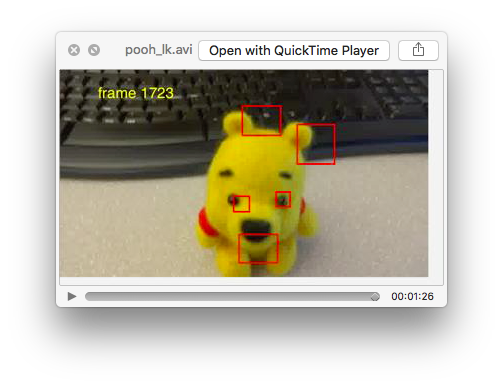
\includegraphics[width=0.6\linewidth]{../matlab/lost_track.png}
  \caption{{\bf My tracker got lost on frame number 2719}, the frame count in the picture starts from frame 992, so the lost track frame is $992+1727 = 2719$}
  \label{lostinspace}
\end{figure}


\subsubsection{Extra Credit (10 pts)\\}

Try modifying the LK tracker such that it can track Winnie the Pooh for more frames. Any techniques or modifications are
welcomed.

Please be sure to describe what you did or tried to do. Make it easy for the marker to give you some extra marks here :)

\subsection{Tracking the Pooh with Supervised Descent Method (SDM) Tracker}

\subsubsection{Training step 1: perturbation (10 pts)\\}

Be sure to include your matlab code using the commented \verb+genPerturbedConfigurations+  below \ldots
\lstinputlisting{../matlab/genPerturbedConfigurations.m}


\subsubsection{Training steps 2\&3: prepare $D$ and $F$ (10 pts)\\}

Be sure to include your matlab code using the commented \verb+genDisplacementMatrix.m+  below \ldots
\lstinputlisting{../matlab/genDisplacementMatrix.m}

Be sure to include your matlab code using the commented \verb+genFeatureMatrix.m+  below \ldots
\lstinputlisting{../matlab/genFeatureMatrix.m}


\subsubsection{Training steps 4\&5: linear mapping and update configuration (10 pts)\\}

Be sure to include your matlab code using the commented \verb+learnMappingAndUpdateConfigurations.m+  below \ldots
\lstinputlisting{../matlab/learnMappingAndUpdateConfigurations.m}


\subsubsection{Sequentially learn multiple mappings (10 pts)\\}

Code for this step is deferred to \verb+SDMtrain.m+ in the next section.


\subsubsection{Integration (15 pts)\\}

Be sure to include your matlab code using the commented \verb+SDMtrain.m+  below \ldots
\lstinputlisting{../matlab/SDMtrain.m}


\subsubsection{Implementation (20 pts)\\}

Be sure to include your matlab code using the commented \verb+SDMtrain.m+  below \ldots
\lstinputlisting{../matlab/SDMtrain.m}

NOTE: The TAs have provided a master script \verb+runTrackPooh_SDM.m+ which runs \verb+SDMtrain.m+ and
\verb+SDMtrack.m+. Please make sure your tracker runs without errors when it is called from
\verb+runTrackPoohSDM.m+. This will be used for grading. Do not modify \verb+runTrackPooh_SDM.m+.

\subsubsection{Discussions (5 pts)}
\label{disc3}

You tried two different trackers on the same sequence. Which one performs better, and why? List two advantages and
disadvantages each for the LK and SDM trackers respectively on this part-based tracking task.

SDM tracker works better than LK tracker.

For SDM tracker:
\begin{enumerate}[I]
\item advantages:
	\begin{enumerate}[(1)]
	\item the convergence rate is quadratic
	\item guaranteed to converge provided that the initial estimate is sufficiently close to the minimum
	\end{enumerate}
\item disadvantages:
	\begin{enumerate}[(1)]
	\item need properly tune parameters to train in different scenarios
	\item lose track for rapid movement
	\end{enumerate}
\end{enumerate}

For LK tracker:
\begin{enumerate}[I]
\item advantages:
	\begin{enumerate}[(1)]
	\item fast
	\item accurate time derivatives
	\end{enumerate}
\item disadvantages:
	\begin{enumerate}[(1)]
	\item errors on boundaries
	\item not robust to changes of illumination, rapid movement
	\end{enumerate}
\end{enumerate}

\subsubsection{Extra credits (3+3+3 pts)}

Write which challenges if any you have overcome here and include the path to your code for fixing this.

Challenge overcome:

(1) over 1410: done.

(2) over 2232: track for the first few frames: done by add large scales for training. 

(3) over 2452: failed.

\subsubsection{Extra credits (10 pts)}

Write about your modifications for dealing with rotation and include a video (and tell us the path here so we find
it!). Be sure to let us know the path to your modified code so we can run it too.


\end{document}
